\chapter{Background}
\label{chapterlabel2}
In this chapter the basic background of the cardiovascular system and computational fluid dynamics will be introduced. Additionally, the process of verification, validation and uncertainty quantification will be explained.


\section{Cardiovascular system}
The cardiovascular system, also called the circulatory system, is a closed-loop system composed by the heart, blood vessels and blood. It uses blood as the medium to distribute oxygen and nutrients to all body tissues and dispose of carbon-dioxide and metabolic waste to lungs and excretory organs. Additionally, the secondary function of the system is to redistribute bioactive agents and hormones throughout the body, and regulate the body temperature \cite{Levick2010Introduction5ed}.\par

The heart is a muscular organ that  pumps the blood into the blood vessels to distribute it around the body. It is located in between the lungs above the sternum. The heart is divided into two sides and each side is divided further into two chambers (as seen on Figure \ref{fig:heart}. The top chambers are the atria and the bottom ones are the ventricles. The wall of the heart are composed of cardiac muscle which produce contraction that pump the blood into the arteries \cite{aaronson2012cardiovascular,tortora2017introduction}. \par

The system is divided into two circulatory loops with heart at the center, a pulmonary circulation and systemic circulation. In the pulmonary circulation, the deoxygenated blood is pumped from the heart's right ventricle into the pulmonary artery, where the blood is transported into the lungs where an oxygen exchange occurs. The blood then returns to the left atrium, passes through the left ventricle into the systematic circulation\cite{Levick2010Introduction5ed,tortora2017introduction}. \par


%The cardiovascular system is a closed-loop system composed of the heart, blood vessels and blood. The main function of the system is to distribute oxygen and other nutrients to all body tissues. Additionally, it also transports carbon-dioxide and other waste products to the lungs and excretory organs \cite{tortora2017introduction, aaronson2012cardiovascular}. The cardiovascular system has also a control function that redistributes hormones and bioactive agents and regulates the body temperature \cite{Levick2010Introduction5ed}.\par

\begin{figure}[ht!]
  \centering
  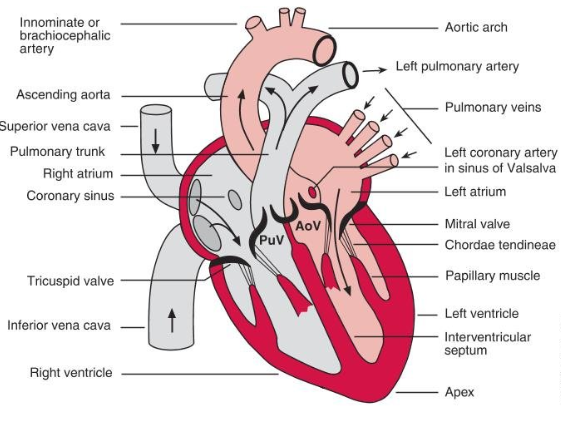
\includegraphics[width=0.6\textwidth]{Figures/heart}
  \caption{Structure of the heart and connection to the major veins and arteries \cite{Levick2010Introduction5ed}.}
  \label{fig:heart}
\end{figure}

%The driving force of the whole system is the heart, which is situated between the lungs behind the sternum above the diaphragm. The heart is divided into a right side and a left side by a layer called septum in between (as seen in Figure \ref{fig:heart}). Each of these sides is made up of two chambers, an atrium and a ventricle. The walls of the heart are composed of cardiac muscle, which generates the contraction and drives the blood flow in and out of the heart. The deoxygenated blood enters the right atrium through the vena cava which then enters the right ventricle through the tricuspid valve and subsequently exits the heart into the pulmonary artery. The blood is then transported to the lungs where an oxygen exchange occurs. The oxygenated blood is then transported back into the left atrium, through the mitral valve into the left ventricle where the blood exits the heart into the aorta \cite{aaronson2012cardiovascular,tortora2017introduction}.\par

The blood vessels of the system are responsible to deliver the blood into organs and tissue. The blood is driven into the aorta from there it flows into the major arteries, which then deliver blood to the major regions and organs. The arteries can further branch out and then they converge into veins which transport the blood back into the heart \cite{Levick2010Introduction5ed}.\par

\subsection{Cardiovascular diseases}



\section{Computational Fluid Dynamics Modelling for cardiovascular applications}
Computational fluid d

\subsection{Governing equations}
Blood is usually described as a continuous and incompressible viscous-fluid. The governing equations of the flow are the Navier-Stokes equations (\ref{eq:n_s}) which describe the conservation of momentum of a fluid. Thus, the flow can be calculated in conjunction with the conservation of mass equation (\ref{eq:con} ):
\begin{equation}
\frac{\partial \rho}{\partial t}+\nabla \cdot (\rho U) = 0 \\
\label{eq:con}
\end{equation}
\begin{equation}
\frac{\partial (\rho U)}{\partial t}+\nabla \cdot (\rho U \times U) = -\nabla p + \nabla \cdot \tau + S_{M}
\label{eq:n_s}
\end{equation}
where, $p$ and $\tau$ are the pressure and stress tensor, respectively and $U$ is the velocity of the flow. The term $S_M$ refers for any momentum of external forces to the system. \par

\subsection{Patient-specific data}
In order to create image-based patient-specific haemodynamics models, it is necessary to obtain geometry and flow data. \par

Imaging techniques such a computed tomography (CT) can be used to obtain a number of image slices which would then be used to reconstruct the 3D model of the tissue and organs of the patient. The method  uses ionising radiation which benefits from high spatial resolution and high penetration depth. However, CT scanning often has limited sensitivity and also exposes the patient to radiation \cite{Saremi2015CoronaryCT}. An alternative method to obtain the geometry can be magnetic resonance imaging (MRI) which uses the principles of electromagnetism to capture the images. It yields the images based on the radiofrequency of the tissue, generated by the hydrogen atoms within the tissues. Using MRI, the patient is not exposed to radiation or contrast agents. However, in comparison with the CT images, the MRI has lower spatial resolution and it is much more time-consuming to acquire whole 3D stack of images \cite{Maurovich-Horvat2012DifferentiationHearts, Karmonik2008ComputationalRates}.\par

Other patient-specific data such as volumetric flow, pressure  or wall motion data has to be obtained in order to create accurate haemodynamic models. There are numerous ways how these can be obtained, both invasively and non-invasively. While invasive methods can provide accurate measurements through the application of different sensors, it is not desirable to use these techniques for diagnostic purposes. Several non-invasive imaging techniques can be employed. Doppler echocardiography or phase contrast (PC) MRI has shown to be a good method for obtaining flow measurements non-invasively \cite{Whitlock2015NoninvasiveAorta}. For the motion of the wall, the time-resolved images must be obtained; this can be done using electrocardiogram (ECG) coupled with CT or 4D MRI data for example \cite{Bonfanti2017ComputationalData,Alimohammadi2015AorticUnderstanding}.

\subsection{Modelling assumptions}

\subsubsection{Viscosity model}
The blood is a complex fluid composed of red and white blood cells and platelets in plasma.\par

While blood exhibits non-Newtonian properties, many of the haemodynamic models assume blood as a Newtonian fluid in large arteries. While the strain rates in these vessels are very low \cite{Fung1997BiomechanicsCirculation}, the Newtonian fluid does not take into account the shear-thinning properties of blood. By increasing the shear rate on the blood, the viscosity decreases (as seen in Figure \ref{fig:visc}) as a result of the disaggregation and the deformation of red blood cells \cite{Gijsen1999TheModel,Cho1991EffectsFlows}. Simple non-Newtonian models, such as Carreau-Yasuda or the Casson model, have been used to approximate the complex behaviour of the blood and to improve the study of the properties of the blood in vessels  \cite{Alimohammadi2015PredictingApproach}. \par

\begin{figure}[ht!]
\centering
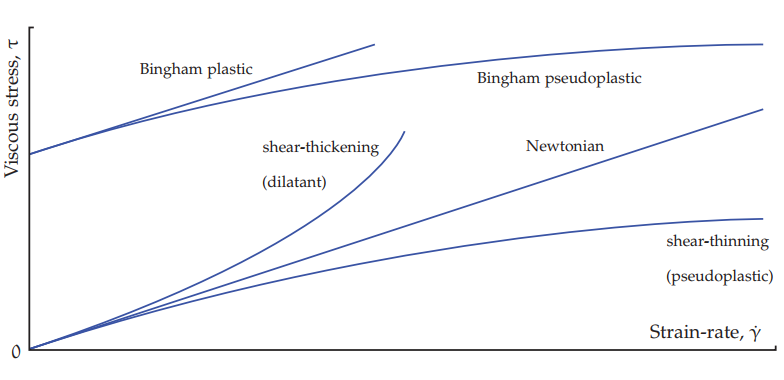
\includegraphics[width=\textwidth]{Figures/viscosity}
\caption{The relation of viscous stress and strain-rate, a comparison of Newtonian and non-Newtonian models \cite{Gabriel2017THEGROWTH}}
\label{fig:visc}
\end{figure}

\subsubsection{Flow models}
Another important consideration to take into account is the flow model which can be laminar, transitional or turbulent \cite{Morris2016ComputationalMedicine}. Turbulent flow introduces random fluctuations in the velocity resulting in turbulent eddies and dissipation of energy in the flow \cite{DongenF.N.vandeVosse2003CardiovascularMechanics}. The Reynold's number $Re$ which is the ratio of the inertial and viscous forces is used to determine the flow regime: 
\begin{equation}
Re = \frac{\rho UD}{\mu}
\end{equation}
Where D is the characteristic length, U is the velocity, $\rho$ is the density and $\mu$ is the viscosity.\par

In a flow, the transition to turbulence occurs at a critical ($Re_c$) of around 2000. The critical Reynold's number $Re$ can be determined using the Womersley number which is the ratio of transient inertial forces to viscous forces. However, it has been shown that in pulsatile flow that occurs in arteries, the $Re_c$ is much higher \cite{Alimohammadi2015PredictingApproach}.\par

A number of studies on the flow conditions in the arteries have found that $Re_c$ varies in the range 2700-15000 and that the maximum Reynolds number in arteries is up to 3700. Therefore, a majority of studies implement the flow as a laminar model. However, in more recent studies, it has been found, that transitional and turbulent regimes can occur in healthy ascending aortae and is more prevalent around aortic diseases \cite{Ku1997BLOODARTERIES}. \par




\section{Verification, validation and uncertainty quantification (VVUQ)}
While computational models can provide a framework to study the complex processes, it is necessary to question the credibility of computational models. The process of assessing models is done in three stages, verification, validation and uncertainty quantification (VVUQ), where different aspects of the models are evaluated. \par

Verification is the assessment of the mathematical and computational reliability. This can involve the assessment of the software quality, design and code review or the numerical analysis of the algorithm used in the code and it's properties (i.e. symmetry, stability, conservation, convergence, etc.). \par

The error of the model is evaluated by validation which compares the numerical results of the model with the true value obtained from the experiments. The process also involved the consideration of the uncertainty that stems from the experiments or from the simulation. 
